\documentclass[border=10pt]{standalone}
\usepackage{tikz}
\usetikzlibrary{positioning, arrows.meta, fit, backgrounds, shadows, calc, decorations.pathreplacing}

\definecolor{appblue}{HTML}{3B82F6}
\definecolor{orchpurple}{HTML}{7C3AED}
\definecolor{infragray}{HTML}{6B7280}
\definecolor{routergreen}{HTML}{059669}
\definecolor{cbred}{HTML}{DC2626}
\definecolor{analyticsamber}{HTML}{D97706}
\definecolor{traceteal}{HTML}{0D9488}
\definecolor{gwblue}{HTML}{2563EB}
\definecolor{gwfib}{HTML}{0891B2}
\definecolor{gwqi}{HTML}{7C3AED}
\definecolor{gwnass}{HTML}{DB2777}
\definecolor{gwcod}{HTML}{65A30D}
\definecolor{gwzain}{HTML}{EA580C}
\definecolor{ifacecolor}{HTML}{8B5CF6}
\definecolor{lightbg}{HTML}{F8FAFC}
\definecolor{extgray}{HTML}{9CA3AF}

\begin{document}
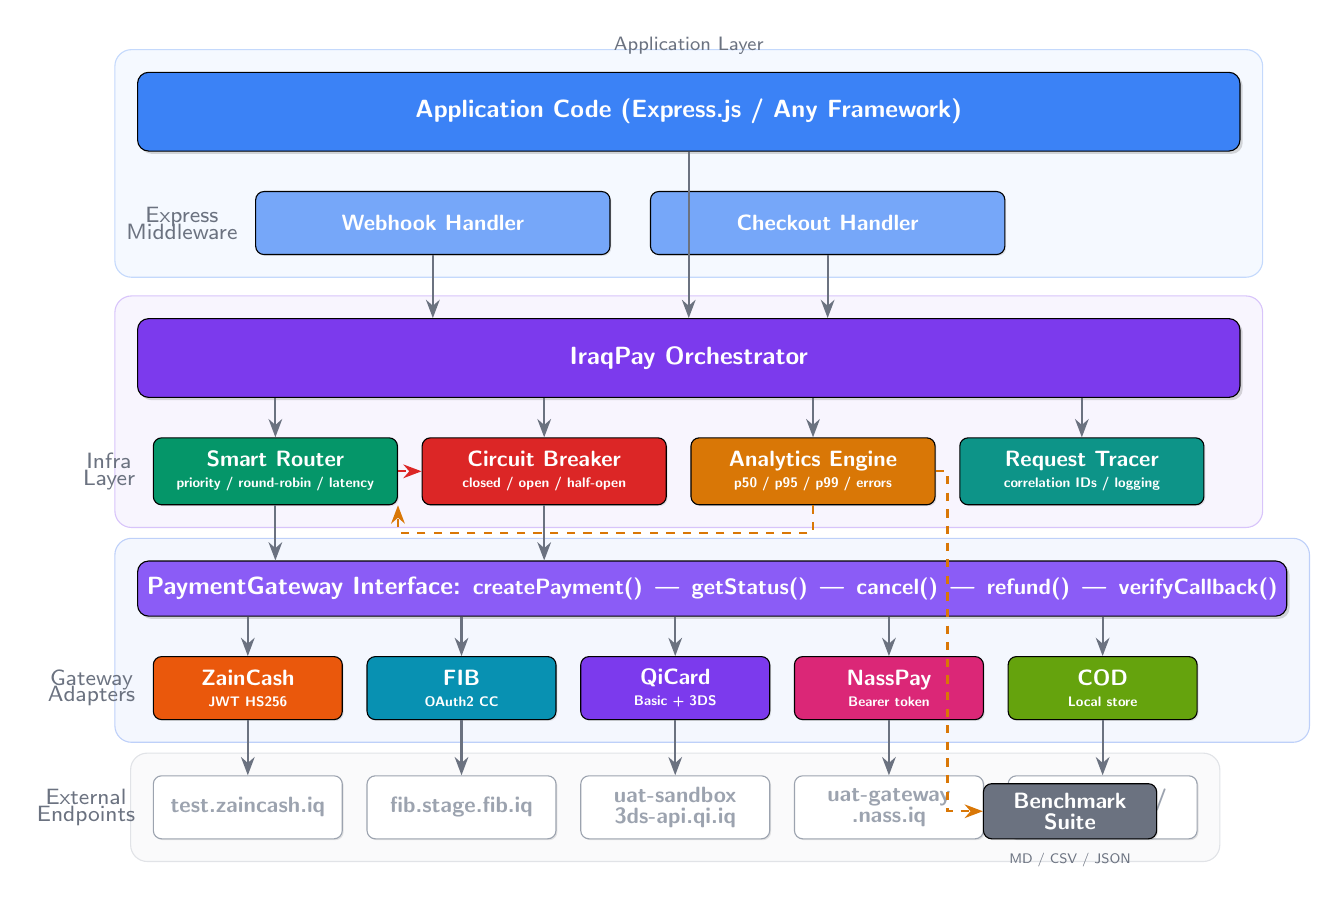
\begin{tikzpicture}[
  >=Stealth,
  node distance=0.6cm,
  every node/.style={font=\sffamily},
  box/.style={
    draw, rounded corners=4pt, minimum height=1.0cm, text=white,
    font=\sffamily\bfseries\small, align=center,
    drop shadow={shadow xshift=1pt, shadow yshift=-1pt, opacity=0.3}
  },
  smallbox/.style={
    draw, rounded corners=3pt, minimum height=0.8cm, minimum width=2.2cm,
    text=white, font=\sffamily\footnotesize\bfseries, align=center,
    drop shadow={shadow xshift=0.5pt, shadow yshift=-0.5pt, opacity=0.2}
  },
  infrabox/.style={
    draw, rounded corners=3pt, minimum height=0.85cm,
    text=white, font=\sffamily\footnotesize\bfseries, align=center,
    drop shadow={shadow xshift=0.5pt, shadow yshift=-0.5pt, opacity=0.2}
  },
  label/.style={font=\sffamily\scriptsize\color{infragray}, align=center},
  arrow/.style={->, thick, color=infragray},
  dataarrow/.style={->, thick, color=analyticsamber, dashed},
]

% ============================================================
% APPLICATION LAYER
% ============================================================
\node[box, fill=appblue, minimum width=14cm] (app)
  {Application Code (Express.js / Any Framework)};

\node[label, above=0.1cm of app] {Application Layer};

% ============================================================
% MIDDLEWARE
% ============================================================
\node[smallbox, fill=appblue!70, below=0.5cm of app.south west, anchor=north west, xshift=1.5cm, minimum width=4.5cm] (webhook)
  {Webhook Handler};
\node[smallbox, fill=appblue!70, right=0.5cm of webhook, minimum width=4.5cm] (checkout)
  {Checkout Handler};

\node[label, left=0.1cm of webhook, anchor=east] {\footnotesize Express\\[-2pt]\footnotesize Middleware};

% ============================================================
% IRAQPAY ORCHESTRATOR
% ============================================================
\node[box, fill=orchpurple, minimum width=14cm, below=0.8cm of webhook.south west, anchor=north west, xshift=-1.5cm] (orchestrator)
  {IraqPay Orchestrator};

% ============================================================
% INFRASTRUCTURE LAYER (4 modules side by side)
% ============================================================
\node[infrabox, fill=routergreen, minimum width=3.1cm,
  below=0.5cm of orchestrator.south west, anchor=north west, xshift=0.2cm] (router)
  {Smart Router\\[-2pt]{\tiny priority / round-robin / latency}};

\node[infrabox, fill=cbred, minimum width=3.1cm, right=0.3cm of router] (cb)
  {Circuit Breaker\\[-2pt]{\tiny closed / open / half-open}};

\node[infrabox, fill=analyticsamber, minimum width=3.1cm, right=0.3cm of cb] (analytics)
  {Analytics Engine\\[-2pt]{\tiny p50 / p95 / p99 / errors}};

\node[infrabox, fill=traceteal, minimum width=3.1cm, right=0.3cm of analytics] (tracer)
  {Request Tracer\\[-2pt]{\tiny correlation IDs / logging}};

\node[label, left=0.1cm of router, anchor=east] {\footnotesize Infra\\[-2pt]\footnotesize Layer};

% ============================================================
% INTERFACE BAR
% ============================================================
\node[box, fill=ifacecolor, minimum width=14cm, below=0.7cm of router.south west, anchor=north west, xshift=-0.2cm, minimum height=0.7cm] (iface)
  {{\small PaymentGateway Interface:} {\footnotesize createPayment() \,|\, getStatus() \,|\, cancel() \,|\, refund() \,|\, verifyCallback()}};

% ============================================================
% GATEWAY ADAPTERS (5 boxes)
% ============================================================
\node[smallbox, fill=gwzain, minimum width=2.4cm,
  below=0.5cm of iface.south west, anchor=north west, xshift=0.2cm] (zain)
  {ZainCash\\[-2pt]{\tiny JWT HS256}};

\node[smallbox, fill=gwfib, minimum width=2.4cm, right=0.3cm of zain] (fib)
  {FIB\\[-2pt]{\tiny OAuth2 CC}};

\node[smallbox, fill=gwqi, minimum width=2.4cm, right=0.3cm of fib] (qi)
  {QiCard\\[-2pt]{\tiny Basic + 3DS}};

\node[smallbox, fill=gwnass, minimum width=2.4cm, right=0.3cm of qi] (nass)
  {NassPay\\[-2pt]{\tiny Bearer token}};

\node[smallbox, fill=gwcod, minimum width=2.4cm, right=0.3cm of nass] (cod)
  {COD\\[-2pt]{\tiny Local store}};

\node[label, left=0.1cm of zain, anchor=east] {\footnotesize Gateway\\[-2pt]\footnotesize Adapters};

% ============================================================
% EXTERNAL SERVICES
% ============================================================
\node[smallbox, draw=extgray, fill=white, text=extgray, minimum width=2.4cm, below=0.7cm of zain] (ezain)
  {test.zaincash.iq};

\node[smallbox, draw=extgray, fill=white, text=extgray, minimum width=2.4cm, below=0.7cm of fib] (efib)
  {fib.stage.fib.iq};

\node[smallbox, draw=extgray, fill=white, text=extgray, minimum width=2.4cm, below=0.7cm of qi] (eqi)
  {uat-sandbox\\[-2pt]3ds-api.qi.iq};

\node[smallbox, draw=extgray, fill=white, text=extgray, minimum width=2.4cm, below=0.7cm of nass] (enass)
  {uat-gateway\\[-2pt].nass.iq};

\node[smallbox, draw=extgray, fill=white, text=extgray, minimum width=2.4cm, below=0.7cm of cod] (ecod)
  {In-memory /\\[-2pt]Database};

\node[label, left=0.1cm of ezain, anchor=east] {\footnotesize External\\[-2pt]\footnotesize Endpoints};

% ============================================================
% BENCHMARK (side)
% ============================================================
\node[infrabox, fill=infragray, minimum width=2.2cm, minimum height=0.7cm,
  right=0.6cm of analytics.east |- ecod.south, anchor=south west] (bench)
  {Benchmark\\[-2pt]Suite};
\node[label, below=0.05cm of bench] {\tiny MD / CSV / JSON};

% ============================================================
% ARROWS — Main flow
% ============================================================
\draw[arrow] (app) -- (orchestrator);
\draw[arrow] (webhook.south) -- ++(0, -0.3) -| (orchestrator.north -| webhook.south);
\draw[arrow] (checkout.south) -- ++(0, -0.3) -| (orchestrator.north -| checkout.south);

% Orchestrator → Infrastructure
\draw[arrow] (orchestrator.south -| router.north) -- (router.north);
\draw[arrow] (orchestrator.south -| cb.north) -- (cb.north);
\draw[arrow] (orchestrator.south -| analytics.north) -- (analytics.north);
\draw[arrow] (orchestrator.south -| tracer.north) -- (tracer.north);

% Infrastructure → Interface
\draw[arrow] (router.south) -- ++(0, -0.2) -| (iface.north -| router.south);
\draw[arrow] (cb.south) -- ++(0, -0.2) -| (iface.north -| cb.south);

% Interface → Gateways
\draw[arrow] (iface.south -| zain.north) -- (zain.north);
\draw[arrow] (iface.south -| fib.north) -- (fib.north);
\draw[arrow] (iface.south -| qi.north) -- (qi.north);
\draw[arrow] (iface.south -| nass.north) -- (nass.north);
\draw[arrow] (iface.south -| cod.north) -- (cod.north);

% Gateways → External
\draw[arrow] (zain.south) -- (ezain.north);
\draw[arrow] (fib.south) -- (efib.north);
\draw[arrow] (qi.south) -- (eqi.north);
\draw[arrow] (nass.south) -- (enass.north);
\draw[arrow] (cod.south) -- (ecod.north);

% Analytics feedback (dashed)
\draw[dataarrow] (analytics.south) -- ++(0, -0.35) -| (router.south east);
\draw[dataarrow] (analytics.east) -- ++(0.15, 0) |- (bench.west);

% Router → CB check
\draw[dataarrow, color=cbred] (router.east) -- (cb.west);

% ============================================================
% BACKGROUND BOXES
% ============================================================
\begin{scope}[on background layer]
  \node[draw=appblue!30, fill=appblue!5, rounded corners=6pt,
    fit=(app)(webhook)(checkout), inner sep=8pt] {};
  \node[draw=orchpurple!30, fill=orchpurple!5, rounded corners=6pt,
    fit=(orchestrator)(router)(cb)(analytics)(tracer), inner sep=8pt] {};
  \node[draw=gwblue!30, fill=gwblue!5, rounded corners=6pt,
    fit=(iface)(zain)(fib)(qi)(nass)(cod), inner sep=8pt] {};
  \node[draw=extgray!30, fill=extgray!5, rounded corners=6pt,
    fit=(ezain)(efib)(eqi)(enass)(ecod), inner sep=8pt] {};
\end{scope}

\end{tikzpicture}
\end{document}
